\section{语法分析——自下而上}

本章开始结构以哈工大教学视频为主。

\subsection{自底向上分析概述}

自底向上分析是从分析树的底部向顶部方向构造分析树,可以看作是将输入串归约为文法开始符的过程。自底向上的语法分析采用\textcolor{mark}{最左规约方式(最右推导)}。

移入-归约分析:

假设有以下输入串 $id + (id+id)$ 以及对应文法:
\begin{equation}
    \begin{aligned}
         & E \rightarrow E+E          \\
         & E \rightarrow E*E          \\
         & E \rightarrow (E)          \\
         & E \rightarrow id \nonumber
    \end{aligned}
\end{equation}

输入串的分析步骤如下:

\begin{table}[H]
    \centering
    \caption{移入-规约分析}
    \label{table:移入-规约分析}
    \setlength{\tabcolsep}{10mm}
    \begin{tabular}{l|r|l}
        \toprule
        \textbf{栈} & \textbf{剩余输入} & \textbf{动作}            \\
        \midrule
        $\#$        & $id+(id+id)\#$    & 预备                     \\
        $\#id$      & $+(id+id)\#$      & 移入                     \\
        $\#E$       & $+(id+id)\#$      & 归约: $E\rightarrow id$  \\
        $\#E+$      & $(id+id)\#$       & 移入                     \\
        $\#E+($     & $id+id)\#$        & 移入                     \\
        $\#E+(id$   & $+id)\#$          & 移入                     \\
        $\#E+(E$    & $+id)\#$          & 归约: $E\rightarrow id$  \\
        $\#E+(E+$   & $id)\#$           & 移入                     \\
        $\#E+(E+id$ & $)\#$             & 移入                     \\
        $\#E+(E+E$  & $)\#$             & 归约: $E\rightarrow id$  \\
        $\#E+(E$    & $)\#$             & 归约: $E\rightarrow E+E$ \\
        $\#E+(E)$   & $\#$              & 移入                     \\
        $\#E+E$     & $\#$              & 归约: $E\rightarrow (E)$ \\
        $\#E$       & $\#$              & 归约: $E\rightarrow E+E$ \\
        $\#E$       & $\#$              & 接受                     \\
        \bottomrule
    \end{tabular}
\end{table}

在这个过程中需要遵循以下几个准则:
\begin{itemize}
    \item 剩余输入从左至右依次移入栈
    \item 栈中从右向左(最右推导)看,能归约则归约
    \item 直到规约为开始符(若不是则出错)
\end{itemize}

上面输入串分析对应的语法树如下:

\begin{figure}[H]
    \centering
    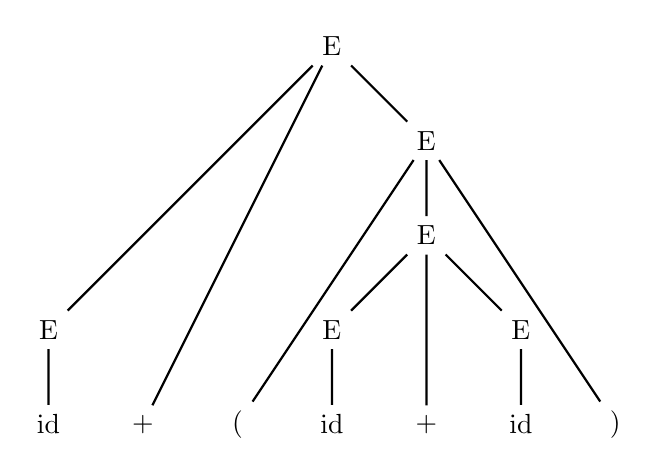
\begin{tikzpicture}[scale = 0.8]
        \node (1-1) at (0,0) {id};
        \node (1-2) at (1.5,0) {+};
        \node (1-3) at (3,0) {(};
        \node (1-4) at (4.5,0) {id};
        \node (1-5) at (6,0) {+};
        \node (1-6) at (7.5,0) {id};
        \node (1-7) at (9,0) {)};
        \node (2-1) at (0,1.5) {E};
        \node (2-2) at (4.5,1.5) {E};
        \node (2-3) at (7.5,1.5) {E};
        \node (3-1) at (6,3) {E};
        \node (4-1) at (6,4.5) {E};
        \node (5-1) at (4.5,6) {E};
        \draw [thick] (1-1) -- (2-1) (1-2) -- (5-1) (1-3) -- (4-1) (1-4) -- (2-2) (1-5) -- (3-1) (1-6) -- (2-3) (1-7) -- (4-1);
        \draw [thick] (2-1) -- (5-1) (2-2) -- (3-1) (2-3) -- (3-1);
        \draw [thick] (3-1) -- (4-1) (4-1) -- (5-1);
    \end{tikzpicture}
    \caption{移入-归约分析语法树}
    \label{移入-归约分析语法树}
\end{figure}

移入-归约分析可能会因为句柄(产生式在语法树中的形式)分析错误而出错(可以匹配多种规约方式)。自底向上分析的关键问题就是如何正确识别句柄。

\subsection{LR 分析法}
\subsubsection{\textcolor{mark}{LR 分析法概述}}

LR 分析法是最大的,可以构造出相应 移入-归约语法分析器的文法类。
\textcolor{mark}{
    \begin{itemize}
        \item L: 对输入进行从左到右扫描
        \item R: 反向构造出一个最右推导序列
        \item LR(k): 向前查看 k 个输入符号
    \end{itemize}
}

句柄是逐步形成的,用 ``状态'' 表示句柄识别的进展程度。例如 $S \rightarrow bBB$ 有以下状态($\cdot$ 前为移入栈的字符)
\begin{equation}
    \begin{aligned}
         & S \rightarrow \cdot bBB & \text{移进状态}           \\
         & S \rightarrow b\cdot BB & \text{待约状态}           \\
         & S \rightarrow bB\cdot B & \text{待约状态}           \\
         & S \rightarrow bBB\cdot  & \text{归约状态} \nonumber
    \end{aligned}
\end{equation}

LR 分析器的总体结构图如下(明天考试了,画的比较草率,可以参考书 P100):

\begin{figure}[H]
    \centering
    \begin{tikzpicture}[font = \small,thick]
        \begin{scope}[inner xsep = 3ex,inner ysep=1ex,text width=3em]
            \node[draw,text width = 5em,inner ysep = 2em] (main) at (0,0) {LR 主控程序};
            \node[draw,text width = 2em] (stack) at (-5,0) {状态栈与符号栈};
            \node[draw,text width = 3em,inner xsep = 4em] (input) at (0,2.5) {输入串};
            \node[draw,text width=4em] (action) at (-2,-2.7) {动作表  ACTION};
            \node[draw,text width=4em] (goto) at (2,-2.7) {转移表  GOTO};
            \node (output) at (5,0) {输出};
        \end{scope}
        \begin{scope}[-Stealth]
            \draw (main) -- (stack);
            \draw (main) -- (input);
            \draw (main) -- (output);
            \draw (main) -- ++(0,-1.5) -| (action);
            \draw (main) -- ++(0,-1.5) -| (goto);
        \end{scope}
    \end{tikzpicture}
    \caption{LR 分析器的总体结构}
    \label{LR 分析器的总体结构}
\end{figure}

LR 分析表结构:

假如有以下文法:
\begin{equation}
    \begin{aligned}
         & S \rightarrow BB           \\
         & B \rightarrow aB           \\
         & B \rightarrow b  \nonumber
    \end{aligned}
\end{equation}

分析表如下,其中:
\begin{itemize}
    \item sn: 将符号 a, 状态 n 压入栈(进行移入操作,并进入状态n)
    \item rn: 用第 n 个产生式进行归约(进行归约操作,使用第 n 个产生式归约)
\end{itemize}

\begin{table}[H]
    \centering
    \caption{LR 分析表结构}
    \label{table:LR 分析表结构}
    \setlength{\tabcolsep}{4mm}
    \begin{tabular}{|c|c|c|c|c|c|c|c|c|}
        \hline
        \multirow{2}{*}{状态} & \multicolumn{3}{c|}{ACTION} & \multicolumn{2}{c|}{GOTO}               \\ \cline{2-6}
                              & a                           & b                         & \#  & S & B \\ \hline
        0                     & s3                          & s4                        &     & 1 & 2 \\ \hline
        1                     &                             &                           & acc &   &   \\ \hline
        2                     & s3                          & s4                        &     &   & 5 \\ \hline
        3                     & s3                          & s4                        &     &   & 6 \\ \hline
        4                     & r3                          & r3                        & r3  &   &   \\ \hline
        5                     & r1                          & r1                        & r1  &   &   \\ \hline
        6                     & r2                          & r2                        & r2  &   &   \\
        \hline
    \end{tabular}
\end{table}

具体的动态演示请看视频: \url{https://www.bilibili.com/video/BV1zW411t7YE?p=27} 这里只说明要点:

\begin{itemize}
    \item 符号栈与状态栈一一对应,归约时同时消去对应的字符和状态。
\end{itemize}

\subsubsection{\textcolor{imp}{LR(0) 分析}}
LR(0) 项目: 右部某位置标有圆点的产生式称为相应文法的一个 LR(0) 项目:
\[S \rightarrow \alpha_1 \cdot \alpha_2\]
\begin{equation}
    \begin{aligned}
         & S \rightarrow \cdot bBB & \text{移进项目:点后为终结符}   &           \\
         & S \rightarrow b\cdot BB & \text{待约项目:点后为非终结符} &           \\
         & S \rightarrow bB\cdot B & \text{待约项目:点后为非终结符} &           \\
         & S \rightarrow bBB\cdot  & \text{归约项目:点后没东西}     & \nonumber
    \end{aligned}
\end{equation}

增广文法: 如果 G 是一个以 S 为开始符号的文法,则 G 的增广文法 $G'$ 就是在 G 中加上新开始符号 $S'$ 和产生式 $S' \rightarrow S$ 而得到的文法。

引入增广文法的目的是使文法开始符号只出现在一个产生式左部,从而使得分析器只有一个接受状态。

后继项目: 接受一个字符后进入下一个项目: 比如 $ S \rightarrow \cdot bBB $ 的后继项目 $S \rightarrow b\cdot BB$ 。

等价项目: 两个项目效果是相同的,比如 $S' \rightarrow \cdot S$ 与 $S \rightarrow \cdot vI$ 中 $S'$ 等待非终结符(要是终结符,就没有等价项目) $S$ 就相当于 $S$ 等待下一个非终结符或终结符。

可以把所有等价的项目组成一个项目集(I),称为项目集闭包,每个项目集闭包对应着自动机的一个状态。构建 LR(0) 自动机需明确以下几个概念:
\begin{itemize}
    \item 项目集闭包: 某个项目及其等价项目构成的集。
    \item 项目集规范族(自动机): 所有项目集闭包构成的全体(项目集以及互相转换关系)。
\end{itemize}

构建自动机(项目集族)的方法见总结与题型。

\subsubsection{\textcolor{mark}{SLR 分析}}

LR(0) 分析过程中的冲突: 项目集中\textcolor{mark}{移进归约冲突}\footnote{LR(0)只有这个冲突,题目问到冲突,找产生式相同的,说是移进规约冲突就行了,下面也类似。},不知道到底用哪个。如果栈顶符号是句柄,应该归约,但是 LR(0) 本身不考虑上下文环境,无法判断。

这个时候要依靠 $FOLLOW$ 集,\textcolor{imp}{如果产生式左部符号的 $FOLLOW$ 集中存在可以进入下一个项目集的符号,那么可以归约,否则不可以。}

SLR 分析法的基本思想:
已知项目集 I 有 m 个移进项目:
\begin{equation}
    \begin{aligned}
         & A_1 \rightarrow \alpha_1 \cdot a_1 \beta_1 \\
         & A_2 \rightarrow \alpha_2 \cdot a_2 \beta_2 \\
         & \cdots                                     \\
         & A_m \rightarrow \alpha_m \cdot a_m \beta_m \\
         & \nonumber
    \end{aligned}
\end{equation}

n 个归约项目:
\begin{equation}
    \begin{aligned}
         & B_1 \rightarrow \gamma_1 \cdot \\
         & B_2 \rightarrow \gamma_2 \cdot \\
         & \cdots                         \\
         & B_n \rightarrow \gamma_n \cdot \\
         & \nonumber
    \end{aligned}
\end{equation}

如果集合 $\{a_1, a_2, \cdots, a_m\}$ 和 $FOLLOW(B_1), FOLLOW(B_2), \dots, FOLLOW(B_n)$ 两两不相交,则项目集 I 中的冲突可以按以下原则解决:
\begin{itemize}
    \item 设 $a$ 是下一个输入符号
    \item 若 $a \in \{a_1,a_2,\cdots,a_m\}$, 则移进 $a$
    \item 若 $a \in FOLLOW(B_i)$, 则用产生式归约
    \item 此外,报错
\end{itemize}

SLR 也叫 SLR(1) ,S 表示简单(Simple), 1 表示向前看一个字符。

如果给定文法的 SLR 分析表中不存在有冲突的动作,那么,该文发称为 SLR 文法。

SLR 分析中的冲突: 移入归约冲突

\subsubsection{\textcolor{imp}{LR(1) 分析}}

SLR 存在的问题: SLR 只是简单地考察下一个输入符号 $b$ 是否属于与规约项目 $A \rightarrow \alpha$ 相关联的 $FOLLOW(A)$, 但 $b \in FOLLOW(A)$ 只是归约 $\alpha$ 的一个必要条件,而非充分条件。

规范 LR(1) 项目:

将一般形式为 $[A \rightarrow \alpha \cdot \beta, a]$ 的项称为 LR(1) 项,其中 $A \rightarrow \alpha \beta$ 是一个产生式, $a$ 是一个终结符(这里将 \# 视为一个特殊的终结符) 它表示在当前状态下,A 后面必须紧跟终结符,称为该项的展望符。

\begin{itemize}
    \item LR(1) 中的 1 指的是项的第二个分量的长度
    \item 在形如 $[A \rightarrow \alpha \cdot \beta ,a]$ 且 $\beta \neq \epsilon$ 的项中,展望符 $a$ 没有任何作用。
    \item 一个形如 $[A \rightarrow \alpha \cdot, a]$ 的项只有在下一个输入符号等于 a 时才可以按照 $A \rightarrow \alpha$ 进行归约 $a$ 的集合总是 FOLLOW(A) 的子集,而且它通常是一个真子集)。
\end{itemize}

等价 LR(1) 项目: 与 LR(0) 类似,$|A \rightarrow \alpha \cdot B\beta ,a|$ 等价于 $|B\rightarrow \cdot \gamma, b|$ 其中 $b \in FIRST(\beta a)$。 当 $\beta \Rightarrow^{+} \epsilon$ 时,此时 $b=a$ 叫继承的后继符,否则叫自生的后继符。

这个后继符比较重要但形式化语言难理解,举个例子(下面几个产生式在一个文法中):
\begin{itemize}
    \item 对于 $S' \rightarrow S$: 它的展望符是 \#, 因为产生式右边 S 后面什么都没有,对应结束符。那么它的 LR(1) 项目为: $S' \rightarrow \cdot S, \#$。
    \item 对于 $S \rightarrow L=R$: $S$ 的展望符继承自上一个式子是 \#, 故它的 LR(1) 项目为: $S \rightarrow \cdot L=R, \#$。
    \item 对于 $L \rightarrow *R$: 在上一个基础上,由于 $L$ 后面有 $=$,根据 $b \in FIRST(\beta a)$,展望符为 $=/\#$,它的 LR(1) 项目为: $L \rightarrow \cdot *R , \#/=$。
\end{itemize}

总而言之,如果某个非终结符后面跟着终结符,则需要加入到对应展望符中\footnote{比较难理解,建议看完视频再理解。}。

针对 LR(1) 也可能出写出项目集族的题目,写法和 LR(0) 非常相似,只需要增加展望符,不再赘述。例子可以参考视频 \url{https://www.bilibili.com/video/BV1zW411t7YE?p=31}。

\subsubsection{\textcolor{imp}{LALR 文法}}

LALR 文法的目的是简化 LR(1) 文法构建的项目集,LALR 文法的基本思想是: 寻找具有相同核心(第一部分)\footnote{去掉展望符的部分。}的 LR(1) 项集,并将这些项集合并为一个项集。

相同核心的项目集称为同心项目集。合并同心项目集时会产生\textcolor{imp}{归约-归约}冲突,不会产生移进-归约冲突,因为展望符只在归约的时候起作用。比如下面归约-归约冲突:

\begin{figure}[H]
    \centering
    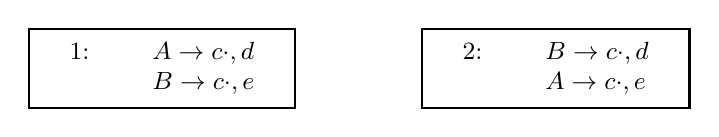
\begin{tikzpicture}[font = \small,thick]
        \node[draw] (0) at (0,0) {
            \begin{tabular}{ll}
                1: & $A \rightarrow c \cdot, d$ \\
                   & $B \rightarrow c \cdot, e$ \\
            \end{tabular}
        };
        \node[draw] (1) at (5,0) {
            \begin{tabular}{ll}
                2: & $B \rightarrow c \cdot, d$ \\
                   & $A \rightarrow c \cdot, e$ \\
            \end{tabular}
        };
    \end{tikzpicture}
    \caption{归约-归约冲突}
    \label{fig:归约-归约冲突}
\end{figure}

合并同心项目集的缺陷:
\begin{itemize}
    \item 引入归约归约冲突
    \item 推迟错误的发现
\end{itemize}

LALR 分析法的特点:
\begin{itemize}
    \item 形式上与 LR(1) 相同
    \item 大小上与 LR(0)/SLR 相同
    \item 分析能力 SLR < LALR(1) < LR(1)
\end{itemize}

\subsubsection{LR 错误处理}

使用二义性文法也不是不行,有时候还能好用,但应该严格控制,因此稍有不慎就会出现偏差\footnote{这原属于二义性文法一节,但知识点太少了,就放在这里。}。

当 LR 分析器在查询分析表并发现一个报错条目时,就检测到一个语法错误。有两种主要的错误恢复策略:
\begin{itemize}
    \item 恐慌模式错误恢复
    \item 短语层次错误恢复
\end{itemize}

\noindent\textbf{恐慌模式错误恢复}

从栈顶向下扫描,直到发现某个状态s,它有一个对应于某个非终结符A的 GOTO 目标,可以认为这个A推导出的串中有错误。

丢弃 0 或多个输入符号,直到发现下一个可能跟在 A 之后的符号为止。

\noindent\textbf{短语层次错误恢复}

检查 LR 分析表中的每一个报错条目,并根据语言的使用方法来决定程序所犯的何种错误最可能引起这个语法错误,然后构造出适当的恢复过程。

\subsection{总结与题型}
\subsubsection{\textcolor{imp}{LR(0)项目集族与分析表}}

构建 LR(0) 自动机的步骤如下\footnote{题目中应该是扣掉某个部分填空,因为项目集编号不统一}:
\begin{itemize}
    \item 构建初始项目的项目集闭包。
    \item 在上一个项目集闭包基础上,以每个项目下一个状态($\cdot$后移)为首个项目,构建项目集闭包。
    \item 重复上一步,直到全部构建规约项目。
\end{itemize}

假设有以下文法:
\begin{equation}
    \begin{aligned}
         & S' \rightarrow S          \\
         & S \rightarrow BB          \\
         & B \rightarrow aB          \\
         & B \rightarrow b \nonumber
    \end{aligned}
\end{equation}

那么他的LR(0)自动机应该为:
\begin{figure}[H]
    \centering
    \begin{tikzpicture}[font = \small,thick]
        \node[draw] (0) at (0,0) {
            \begin{tabular}{ll}
                0: & $S' \rightarrow \cdot S$ \\
                   & $S \rightarrow \cdot BB$ \\
                   & $B \rightarrow \cdot aB$ \\
                   & $B \rightarrow \cdot b$  \\
            \end{tabular}
        };
        \node[draw] (1) at (5,4) {
            \begin{tabular}{ll}
                1: & $S' \rightarrow S\cdot$ \\
            \end{tabular}
        };
        \node[draw] (2) at (5,2) {
            \begin{tabular}{ll}
                2: & $S \rightarrow B\cdot B$ \\
                   & $B \rightarrow \cdot aB$ \\
                   & $B \rightarrow \cdot b$  \\
            \end{tabular}
        };
        \node[draw] (3) at (5,-1) {
            \begin{tabular}{ll}
                3: & $B \rightarrow a\cdot B$ \\
                   & $B \rightarrow \cdot aB$ \\
                   & $B \rightarrow \cdot b$  \\
            \end{tabular}
        };
        \node[draw] (4) at (5,-3) {
            \begin{tabular}{ll}
                4: & $B \rightarrow b\cdot$ \\
            \end{tabular}
        };
        \node[draw] (5) at (10,2) {
            \begin{tabular}{ll}
                5: & $S \rightarrow BB\cdot$ \\
            \end{tabular}
        };
        \node[draw] (6) at (10,-1) {
            \begin{tabular}{ll}
                6: & $B \rightarrow aB\cdot$ \\
            \end{tabular}
        };
        \begin{scope}[-Stealth]
            \draw (0) to[out = 60,in = 180] node [pos=0.5,above] {S} (1);
            \draw (0) to[out = 30,in = 180] node [pos=0.5,above] {B} (2);
            \draw (0) to[out = -30,in = 180] node [pos=0.5,above] {a} (3);
            \draw (0) to[out = -60,in = 180] node [pos=0.5,above] {b} (4);
            \draw (2) to[out = 0,in = 180] node [pos=0.5,above] {B} (5);
            \draw (2) to[out = -90,in = 90] node [pos=0.5,left] {a} (3);
            \draw (2) to[out = -15,in = 15] node [pos=0.5,left] {b} (4);
            \draw (3) to[out = 0,in = 180] node [pos=0.7,above] {B} (6);
            \draw (3) to[out = 0,in = -15] node [pos=0.5,right] {a} (3);
            \draw (3) to[out = -90,in = 90] node [pos=0.5,right] {b} (4);
        \end{scope}
    \end{tikzpicture}
    \caption{LR(0)自动机}
    \label{fig:LR(0)自动机}
\end{figure}

有了转换图就可以构建转换表:

\begin{table}[H]
    \centering
    \setlength{\tabcolsep}{4mm}
    \begin{tabular}{|c|c|c|c|c|c|c|c|c|}
        \hline
        \multirow{2}{*}{状态} & \multicolumn{3}{c|}{ACTION} & \multicolumn{2}{c|}{GOTO}               \\ \cline{2-6}
                              & a                           & b                         & \#  & S & B \\ \hline
        0                     & s3                          & s4                        &     & 1 & 2 \\ \hline
        1                     &                             &                           & acc &   &   \\ \hline
        2                     & s3                          & s4                        &     &   & 5 \\ \hline
        3                     & s3                          & s4                        &     &   & 6 \\ \hline
        4                     & r3                          & r3                        & r3  &   &   \\ \hline
        5                     & r1                          & r1                        & r1  &   &   \\ \hline
        6                     & r2                          & r2                        & r2  &   &   \\
        \hline
    \end{tabular}
\end{table}

\includegraphics[width=16cm]{../figures/5.语法分析.pdf}


\includegraphics[width=16cm]{../figures/题目构造LR文法的分析表.pdf}


\newpage